%!TEX root = ..//Avali-Arena-Esportivas.tex

\section{ANÁLISE DO TRATAMENTO ESTATÍSTICO - CUSTO BENFEITORIAS / TERRENO}

\subsection{AMOSTRA ESTÁDIO - CUSTO BENFEITORIAS}
%
\hspace*{1.25 cm} Para o tratamento estatístico (tratamento científico com modelos de regressão linear) no cálculo do valor da construção, foi realizado com o software SisDEA. A amostra utilizada é composta de 16 (dezesseis) dados efetivamente usados, descritos.\\ 
%
\hspace*{1.25 cm} Convém ressaltar que foram adotadas, além da variável dependente, 3 (três) variáveis independentes.\\ 
%
\hspace*{1.25 cm} Conforme já mencionado, foram adotadas, no tratamento estatístico científico, quatro variáveis independentes, ou explicativas, as quais são descritas a seguir:
\begin{description}[itemsep=1pt,parsep=1pt]\vspace{0.00mm} 
	\item[DT (data)]  : variável quantitativa aplicada para indicar a data (ano) de inauguração de cada estádio pesquisado.
	\item[T1 (Padrão 1)]  : Variável dummy, ou dicotômica, aplicada para indicar Código 1 = Arena que possui vários espaços multiusos como: área para treinamentos, convenções, lançamento de produtos, formaturas, festas infantis, restaurantes barbearia, lounge temáticos, halls, camarotes diversos, coworking, shows e inovações tecnológicas como reconhecimento facial, telões de LED, controle de acesso.
	\item[T2 (Padrão 2)]  : Variável dummy, ou dicotômica, Código 0 = Arena que possui alguns espaços multiusos dentre os contemplados no código 1.
	\item[R\$/ASSENTO]  : Variável dependente, ou variável a ser explicada, representa o custo de construção de cada estádio por número de lugares (assentos), ou seja, o custo total de construção, dividido pelo número total de assentos. 
\end{description}
%
\begin{table}[h!t]
	\centering
	\begin{threeparttable}
		\caption{Atributos de Entrada do Terreno Avaliado }
		\label{Tabela-variaveis}
		\begin{tabular}{p{13cm}lp{5cm} l}
			\toprule
			Variável & Atributo    	 \\\midrule
			N de Assentos	& 50.000,00 	 \\	 
			Tipo de Arena	& 0 \\	 
			Data de Inauguração	&12      \\\bottomrule
		\end{tabular}%
		\begin{tablenotes}
			\item [{\normalsize Fonte:     Elaborado pelos Autores (2025)}]  
		\end{tablenotes}
	\end{threeparttable}
\end{table}
\hspace*{1.25 cm} Em relação às duas variáveis dicotômicas, é importante destacar que foram identificados, na amostra, três padrões distintos de estádios esportivos. As duas variáveis dicotômicas adotadas foram suficientes para explicar as diferenças entre os padrões existentes, uma vez que, se P1 e P2 assumirem a posição “não”, resta então o terceiro padrão identificado, referente à estádios esportivos com estrutura tecnológica básica, não preparados para múltiplos usos.
%
%

\begin{longtable}[c]{p{1cm}lp{4cm}l l l lp{3cm}l}
	\caption{Amostra do Tratamento Estatístico da construção.}\\ \toprule
	Item & Endereço & Informante & T1 & T2 &Data &R\$ / Assento    \\ 
	\endfirsthead
	\multicolumn{6}{c} {{\tablename\ \thetable{} -- Contin\'ua na p\'agina anterior}} \\    \toprule
	Item & Endereço & Informante & T1 & T2 &Data &R\$ / Assento    \\  \midrule
	\endhead
	\midrule
	%	\multicolumn{6}{r}{{Contin\'ua na pagina seguinte...}}\\ \midrule
	\endfoot
	\bottomrule
	%Item & Endereço & Informante & T1 & T2 &Data &R\$ / Assento    	 \\
	1&	Grêmio	&http	"stadiumdb.com	&0	&0	&3	&8.919,72\\ 
	2&	Allianz Parque	&http	"stadiumdb.com	&1&	0	&3&	14.412,19\\ 
	3&	Engenhão&	http	"stadiumdb.com	&0&	0&	6	&8.508,54\\ 
	4&	Maracanã&	http	"stadiumdb.com	&1&	0&	2&	14.460,03\\ 
	5&	Arena Pantanal&	http	//stadiumdb.com	&1	&0&	3	&15.607,63\\ 
	6&	Amazônia&	http	//stadiumdb.com	&1&	0&	3&	15.095,49\\ 
	7&	Arena das Dunas	&http	//stadiumdb.com	 &1	&0&	3	&13.482,07\\ 
	8&	Beira-Rio&	http	//stadiumdb.com&	0&	0&	3	&6.370,66\\ 
	9&	Estádio Pedro &http	//stadiumdb.com&	0&	0&	5	&7.111,11\\ 
	10&	Novo Castelão&	http	//stadiumdb.com	&0&1	&2	&8.115,42\\ 
	11	&Arena Pernambuco&	http	//stadiumdb.com& 1&	0&	2	&14.083,29\\  
	12&	Arena MRV &http	//stadiumdb.com&	0&	1&	11	&11.798,17\\ 
	13&Arena do Esporte&http	//stadiumdb.com	&0	&1	&5	&13.043,48\\ 
	14	&Urbano Caldeira&	http	//stadiumdb.com&0&	1&	14	&14.946,13\\  
	15&Independência&http	//stadiumdb.com	&0	&0	&1	&5.212,21\\ 
	16&Arena da Baixada&http	//stadiumdb.com&0&0&2&8.700,91\\  
\end{longtable}
Fonte:     Elaborado pelos Autores (2025)

\subsection{MODELO ESTATÍSTICO DO TRATAMENTO CIENTÍFICO - SisDEA}
\begin{table}[h!t]
	\centering
	\begin{threeparttable}
		\caption{Atributos de Entrada do Terreno Avaliado }
		\label{Tabela-variavedis}
		\begin{tabular}{lll}
			\toprule
			\multicolumn{3}{l}{Modelo do SisDea}                   \\\midrule
			Modelo                & XXX               &             \\
			Data da criação       & 16/02/025         &             \\
			Área de concentração  & Avaliação de Bens &             \\
			Tipologia em estudo   & Outras            &             \\
			Dados do Modelo       & 16                &             \\
			Dados utilizados      & 4                 &             \\
			Variáveis utilizadas  & 4                 &             \\
			& Regressão         & Estimativa  \\
			Coef. de correlação   & 0,937227481       & 0,945805744 \\
			Coef. de determinação & 0,878395351       & 0,894548505 \\
			Desvio Padrão         & 0,138222614       & 1295,022687 \\
			&                   &             \\
			Normalidade:          & \multicolumn{2}{c}{68,93,100}    \\\bottomrule
		\end{tabular}
		\begin{tablenotes}
			\item [{\normalsize Fonte:     Elaborado pelos Autores (2025)}]  
		\end{tablenotes}
	\end{threeparttable}
\end{table}

\begin{comment}
	| Modelo do SisDEA |		\\ 
	Modelo:	XXXXXXX	\\ 
	Data de criação:	16/02/2025	\\ 
	Área de concentração:	Avaliação de Bens	\\ 
	Tipologia em estudo:	Outras	\\ 
	Dados do modelo:	16	\\ 
	Dados utilizados:	16	\\ 
	Variáveis do modelo:	4	\\ 
	Variáveis utilizadas:	4	\\ 
	\\ 
	Regressão	Estimativa\\ 
	Coef. de correlação	0,937227481	0,945805744\\ 
	Coef. de determinação	0,878395351	0,894548505\\ 
	Desvio padrão	0,138222614	1295,022687\\ 	 
\end{comment}

\subsubsection{RESULTADOS}

\begin{minipage}[t!]{0.5\textwidth}
	\begin{figure}[H]
		\centering  \small 		\caption{ Resultados pelo SISDEA}
		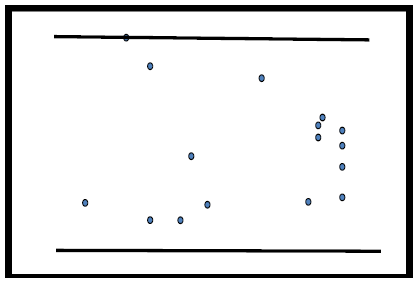
\includegraphics[width=0.9347\linewidth]{figura/screenshot030}
		\label{fig:screenshot030}
	\end{figure}
	
\end{minipage}\hfill
\begin{minipage}[t!]{0.5\textwidth}
	\begin{figure}[H]
		\centering  \small 		\caption{ Resultados pelo SISDEA}
		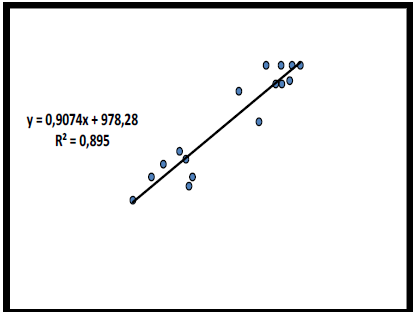
\includegraphics[width=0.9347\linewidth]{figura/screenshot031}
		\label{fig:screenshot031}
	\end{figure}
\end{minipage} 
\begin{center}
	Fonte: Elaborado pelos Autores, pelo SISDEA
\end{center}

\begin{figure}[H]
	\centering  \small 		\caption{ Resultados pelo SISDEA}
	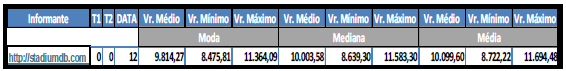
\includegraphics[width=0.947\linewidth]{figura/screenshot032}
	\label{fig:screenshot032}\\{ Fonte: Elaborado pelos Autores, pelo SISDEA}
\end{figure}


\begin{comment}
	%
	\hspace*{1.25 cm} Caracterização do im óvel avaliando	Completa quanto a todas as variáveis analisadas	Completa quanto às Adoção de situação variáveis utilizadas no modelo paradigma	3\\ 
	%
	\hspace*{1.25 cm} Quantidade mínima de dados de mercado, efetivamente utilizados	6 (k+1), onde k é o número de variáveis independentes	4 (k+1), onde k é o 3 (k+1), onde k é o número de variáveis número de variáveis independentes independentes	2\\ 
	%
	\hspace*{1.25 cm} Identificação dos dados de Imdeenrctaifdicoação dos dados de	Apresentação de informações relativas a todos os dados e variáveis analisados na modelagem, com foto e características observadas pelo autor do laudo	Apresentação de Apresentação de informações relativas a informações relativas todos os dados e aos dados e variáveis variáveis analisados na efetivamente utilizados modelagem no modelo	3\\ 
	—	Não admitida	Admitida, desde que: Admitida para apenas a) as medidas das uma variável, desde características do imóvel que: a) as medidas das avaliando não sejam características do imóvel superiores a avaliando não sejam 100 \% do limite superiores a 100\% do amostral superior, nem nem inferiores à limite amostral inferior metade do limite b) o valor estimado não amostral inferior, b) o ultrapasse 20 \% do valor valor estimado não calculado no limite da ultrapasse 15\% do valor fronteira amostral, para calculado no limite da as referidas variáveis, de fronteira amostral, para per si e a referida variável simultaneamente, e em módulo	3\\ 
	Nível de significância (som atório do valor das duas caudas) máximo para a rejeição da hipótese nula de cada regressor (teste bicaudal)	10\%	20\% 30\%	3\\ 
	Nível de significância máximo admitido para a rejeição da hipótese nula do modelo através do teste F de Snedecor	1\%	2\% 5\%	\\ 
	10 6	17\\ 
	2, 4, 5 e 6 no grau III e os demais no mínimo no	2, 4, 5 e 6 no mínimo no  , ,. Todos, no mínimo no grau II e os dem ais no grau I mínimo no grau I	\\ 
	Grau de Fundamentação do Laudo				 
\end{comment}

\begin{figure}[H]
	\centering  \small 		\caption{ Resultados pelo SISDEA}
	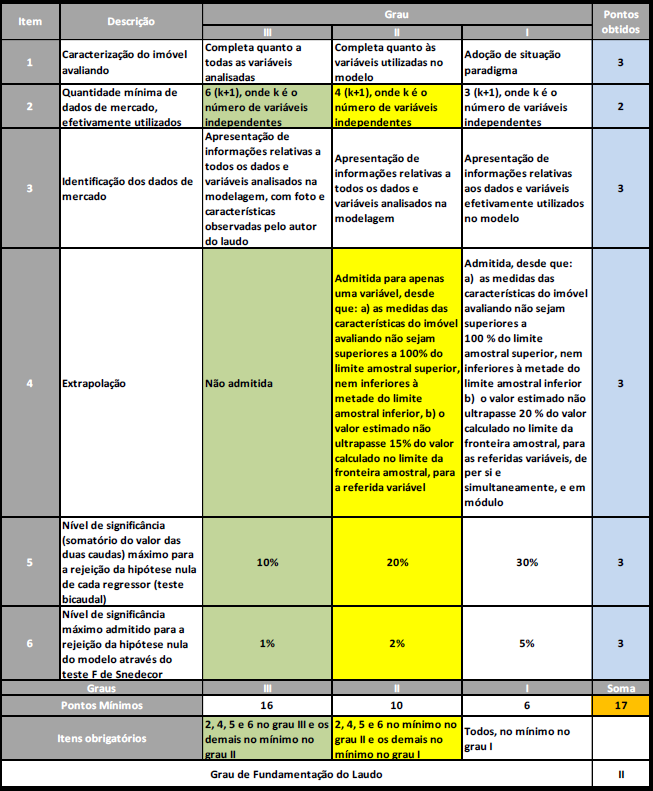
\includegraphics[width=0.947\linewidth]{figura/screenshot033}
	\label{fig:screenshot033}\\{ Fonte: Elaborado pelos Autores, pelo SISDEA}
\end{figure}

\subsection{AMOSTRA ESTÁDIO VALOR DO TERRENO}
%
\hspace*{1.25 cm} Para o tratamento estatístico (tratamento científico com modelos de regressão linear) no cálculo do valor da construção, foi realizado com o software SisDEA. A amostra utilizada é composta de 46 (quarenta e seis) dados efetivamente usados, descritos no item 2 deste trabalho.\\ 
%
\hspace*{1.25 cm}  Convém ressaltar que foram adotadas, além da variável dependente, 4 (quatro) variáveis independentes.\\ 
%
\hspace*{1.25 cm}  Conforme já mencionado, foram adotadas, no tratamento estatístico científico, quatro variáveis independentes, ou explicativas, as quais são descritas a seguir:
%
\begin{description}[itemsep=1pt,parsep=1pt]\vspace{0.00mm} 
	\item[\textbf{Valor / m2}]   - Variável dependente ou explicada. Valor que queremos calcular. Identifica o valor total dividido pela área total do imóvel.
	
	\item[\textbf{Área total}]   - Variável independente quantitativa das áreas totais dos terrenos pesquisados. A hipótese formulada busca mostrar que quanto maior a área menor o valor unitário, tendo em vista as leis de mercado.
	
	\item[\textbf{Indice fiscal (PMS)}]   - Variável independente proxy que indica a proporção do Índice Fiscal da Prefeitura Municipal do Salvador dos imóveis pesquisados. A hipótese formulada busca mostrar que quanto maior a atratividade maior o valor unitário.
	
	\item[\textbf{Vocação} ]  - Variável independente qualitativa representada por códigos alocados, que indica a vocação dos imóveis pesquisados, sendo: 1 = Residencial Unifamiliar; 2 = Residencial Multifamiliar e 3 = Comercial.
	
	\item[\textbf{CAB PDDU}]   - Variável independente proxy que indica o CAB dos imóveis pesquisados. A hipótese formulada busca mostrar que quanto maior a atratividade maior o valor unitário
\end{description}


\begin{table}[ht]
	\centering
	\begin{threeparttable}
		\caption{Atributos de Entrada do Terreno Avaliado }
		\label{Tabela-entrada-avaliado}
		\begin{tabular}{p{13.0cm}l  l}
			\toprule
			Variavel & Atributo    	 \\\midrule
			Area total	& 129.277,00 	 \\	 
			Setor Urbano	& 45,07 \\	 
			Vocacao	&3     \\	 
			CAB	& 1,05    \\\bottomrule
		\end{tabular}%
		\begin{tablenotes}
			\item [{\normalsize Fonte:     Elaborado pelos Autores (2025)}]  
		\end{tablenotes}
	\end{threeparttable}
\end{table}

\subsection{MODELO ESTATÍSTICO DO TRATAMENTO CIENTÍFICO - SisDEA}

\begin{table}[h!t]
	\centering
	\begin{threeparttable}
		\caption{Resultado do Terreno Avaliado }
		\label{Tabela-entrada-avalia5do}
		\begin{tabular}{p{2.5cm}lp{1.0cm}lp{2.5cm}lp{1.0cm}lp{1.5cm}lp{2.0cm}lp{1.0cm}lp{1.0cm}ll}
			\toprule
			Variável&	Média&	Mínimo&	Máximo&	Coeficiente&	t&	Sig(\%)	&transf 	 \\\midrule
			Área total&	86,34&	18,97&	367,42&	0,00&	4,84&	0,00&	th\\ 
			Índice Fiscal (PMS)&	0,03&	0,01&	0,08&	0,25&	8,11	&0,00&	1/x\\ 
			Vocação	&2,33&	1,00&	3,00&	0,00&	-6,22&	0,00&	x\\ 
			CAB (PDDU)	&1,38&	0,50&	2,00&	-0,01&	-11,04&	0,00&	x\\ 
			Valor Unitário	&0,03&	0,01&	0,04&	0,04&	20,31&	0,00	&1/yh \\\bottomrule
		\end{tabular}%
		\begin{tablenotes}
			\item [{\normalsize Fonte:     Elaborado pelos Autores (2025)}]  
		\end{tablenotes}
	\end{threeparttable}
\end{table}

\begin{table}[h!t]
	\centering
	\begin{threeparttable}
		\caption{Resultado do Terreno Avaliado }
		\label{Tabela-entrada-avaliafd5do}
		\begin{tabular}{p{3.0cm}lp{1.0cm}lp{2.0cm}lp{2.0cm}lp{1.5cm}l}
			\toprule
			\multicolumn{5}{c}{Análise da Variância} 	\\ \midrule
			Fonte de Variação &Soma  dos Quadrados &Graus de Liberdade& Quadrado Médio &F \par calculado\\  \midrule
			Explicada	&0,001535576&	4&	0,00038389&57,09	\\ 
			Não \par  explicada & 0,00027568	&41	&6,72 E-06	& 	\\ 
			Total&	0,001811257	&45	 & & & \\\bottomrule
		\end{tabular}%
		\begin{tablenotes}
			\item [{\normalsize Fonte:     Elaborado pelos Autores (2025)}]  
		\end{tablenotes}
	\end{threeparttable}
\end{table}



\begin{minipage}[t!]{0.5\textwidth}
	\begin{figure}[H]
		\centering  \small 		\caption{ Resultados pelo SISDEA}
		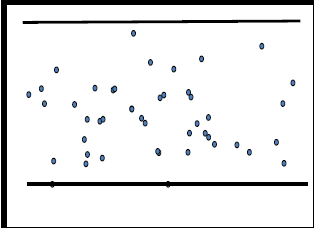
\includegraphics[width=0.93947\linewidth]{figura/screenshot036}
		\label{fig:screenshot036}
	\end{figure}
\end{minipage}\hfill
\begin{minipage}[t!]{0.5\textwidth}
	\begin{figure}[H]
		\centering  \small 		\caption{ Resultados pelo SISDEA}
		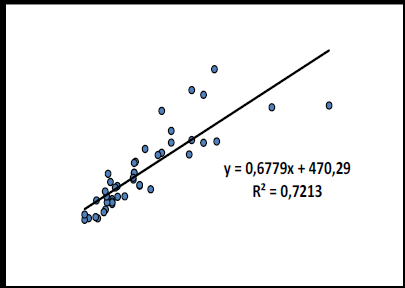
\includegraphics[width=0.93947\linewidth]{figura/screenshot035}
		\label{fig:screenshot035}
	\end{figure}
\end{minipage} 
\begin{center}
	Fonte: Elaborado pelos Autores, pelo SISDEA
\end{center}





\subsubsection{ESTIMATIVAS}

\begin{table}[ht]
	\centering
	\begin{threeparttable}
		\caption{Amostra do Tratamento Estatístico do Custo das Benfeitorias }
		\label{Tabela-e1}
		\begin{tabular}{lp{2.0cm} lp{2.5cm} l p{1.0cm}l p{2.5cm}lp{2.0cm} lp{1.5cm} l}
			\toprule
			Area total &	Índ. Fiscal (PMS)	&Vocação &CAB (PDDU)&	Vr. Médio&	Vr. Mínimo&	Vr. Máximo\\\midrule
			129.277,00&	45,07&	3&	1,5	&1.126,96&	985,20&	1.301,67\\ \bottomrule
		\end{tabular}%
		\begin{tablenotes}
			\item [{\normalsize Fonte:     Elaborado pelos Autores (2025)}]  
		\end{tablenotes}
	\end{threeparttable}
\end{table}
\begin{comment}
	
	
\end{comment}
\begin{figure}[H]
	\centering  \small 		\caption{ Amostra do Tratamento Estatístico do terreno}
	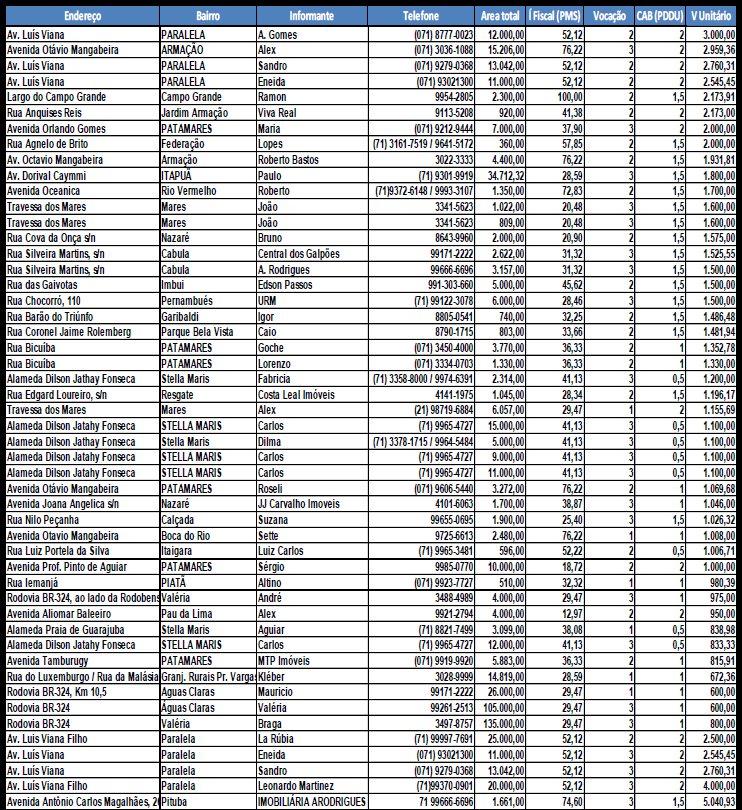
\includegraphics[width=0.947\linewidth]{figura/screenshot037}
	\label{fig:screenshot037}\\{ Fonte: Elaborado pelos Autores, pelo SISDEA}
\end{figure}

\begin{comment}
	\newpage
	\begin{landscape}
		\begin{longtable}[c]{p{2cm}p{1.5cm}lp{1.0cm}lp{0.5cm}lp{0.5cm}lp{0.5cm}lp{0.5cm}lp{0.5cm}lp{0.5cm}lp{0.5cm}l}
			\caption{Tabla de varias p\'aginas con encabezado y pie.}\\ \toprule
			Endereço	&Bairro&	Informante	&Telefone&	Área total& Fiscal \par (PMS)&Vocação&(PDDU)& V Unitário \\ \midrule
			\endfirsthead
			\multicolumn{9}{c} {{\tablename\ \thetable{} -- continua de la p\'agina		anterior}} \\    \toprule
			Endereço	&Bairro&	Informante	&Telefone&	Área total& Fiscal \par (PMS)&Vocação&(PDDU)& V Unitário \\ \midrule
			\endhead
			\midrule
			\multicolumn{9}{r}{{Contin\'ua en la siguiente p\'agina...}}\\ \midrule
			\endfoot
			\bottomrule
			%\endlasthead
			%Endereço	&Bairro&	Informante	&Telefone&	Área total& Fiscal \par (PMS)&Vocação&(PDDU)& V Unitário	 \\\midrule
			Av. Luís Viana&	Paralela&	A. Gomes&	(071) 8777-0023	&12.000,00&52,12&	2&	2&	3.000,00\\ 
			Avenida Otávio Mangabeira&	ARMAÇAO	Alex&	(071) 3036-1088&	15.206,00&	76,22	&3	&2	&2.959,36\\ 
			Av. Luís Viana	&PARALELA	Sandro&	(071) 9279-0368	&13.042,00&	52,12&	2	&2	&2.760,31\\ 
			Av. Luís Viana	&PARALELA	Eneida	&071) 93021300	&11.000,00	&52,12&	2&	2&	2.545,45\\ 
			Largo do Campo Grande	&Campo Grande	Ramon&	9954-2805&	2.300,00&	100,00	&2&	1,5	2.173,91\\ 
			Rua Anquises Reis&	Jardim Armação	Viva Real&	9113-5208&	920,00&	41,38&	2&	2&	2.173,00\\ 
			Avenida Orlando Gomes	&PATAMARES	Maria&	(071) 9212-9444	&7.000,00v	37,90	&3	2&	2.000,00\\ 
			Rua Agnelo de Brito	&Federação	Lopes	&(71) 3161-7519 / 9641-5172	&360,00	&57,85&	2&	1,5	&2.000,00\\ 
			Av. Octavio Mangabeira	&Armação&	Roberto Bastos&	3022-3333	&4.400,00	&76,22&	2&	1,5	1.931,81\\ 
			Av. Dorival Caymmi	&ITAPUA	Paulo&	(71) 9301-9919	&34.712,32&	28,59&	3&	1,5	&1.800,00\\ 
			Avenida Oceanica&	Rio Vermelho&	Roberto	&(71)9372-6148 / 9993-3107&	1.350,00&	72,83&	2&	1,5&	1.700,00\\ 
			Travessa dos Mares	&Mares	João&	3341-5623&	1.022,00&	20,48 	3&	1,5	&1.600,00\\ 
			Travessa dos Mares	&Mares	João&	3341-5623	&809,00&	20,48	&3&	1,5	&1.600,00\\ 
			Rua Cova da Onça s/n&	Nazaré	Bruno&	8643-9960&	2.000,00&	20,90&	2&	1,5&	1.575,00\\ 
			Rua Silveira Martins, s/n	&Cabula	Central dos Galpões	&99171-2222	&2.622,00&	31,32	3	&1,5&	1.525,55\\ 
			Rua Silveira Martins, s/n&	Cabula&	A. Rodrigues&	99666-6696&	3.157,00&	31,32&	3&	1,5&	1.500,00\\ 
			Rua das Gaivotas&	Imbui	&Edson Passos&	991-303-660	&5.000,00&	45,62	2&	1,5	&1.500,00\\ 
			Rua Chocorró, 110	&Pernambués	URM	&(71) 99122-3078	&6.000,00&	28,46	&3	&1,5&	1.500,00\\ 
			Rua Barão do Triúnfo&	Garibaldi&	Igor	&8805-0541&	740,00	&32,25	2	&1,5	&1.486,48\\ 
			Rua Coronel Jaime Rolemberg	&Parque Bela Vista	&Caio	&8790-1715&	803,00	&33,66&	2&	1,5	&1.481,94\\ 
			Rua Bicuíba	PATAMARES&	Goche&	(071) 34504000&	3.770,00&	36,33&	2&	1	&1.352,78\\ 
			Rua Bicuíba	PATAMARES&	Lorenzo&	(071) 3334-0703	&1.330,00&	36,33	&2	&1&	1.330,00\\ 
			Alameda Dilson Jathay Fonseca&	Stella Maris	&Fabricia&	(71) 3358-8000 / 9974-6391	&2.314,00&	41,13	3&	0,5	&1.200,00\\ 
			Rua Edgard Loureiro, s/n	&Resgate&	Costa Leal Imóveis	&4141-1975&1.045,00	28,34&	2	&1,5&	1.196,17\\ 
			Travessa dos Mares	Mares&	Alex &	(21) 98719-6884	&6.057,00	&29,47&	1&	2	&1.155,69\\ 
			Alameda Dilson Jatahy Fonseca&	STELLA MARIS&	Carlos	(71) 99654727&	15.000,00&	41,13&	3&	0,5	&1.100,00\\ 
			Alameda Dilson Jathay Fonseca	&Stella Maris&	Dilma&	(71) 3378-1715 / 9964-5484&	5.000,00&	41,13&	3&	0,5	&1.100,00\\ 
			Alameda Dilson Jatahy Fonseca&	STELLA MARIS&	Carlos	(71) 99654727&	9.000,00&	41,13	&3	&0,5&	1.100,00\\ 
			Alameda Dilson Jatahy Fonseca&	STELLA MARIS&	Carlos&	(71) 99654727	&11.000,00&	41,13&	3&	0,5&	1.100,00\\ 
			Avenida Otávio Mangabeira	&PATAMARES&	Roseli	&(071) 9606-5440&	3.272,00&	76,22	&2	&1	&1.069,68\\ 
			Avenida Joana Angelica s/n	&Nazaré	JJ Carvalho Imoveis 	4101-6063	&1.700,00&	38,87&	3&	1&	1.046,00\\ 
			Rua Nilo Peçanha&	Calçada	Suzana	99655-0695	&1.900,00&	25,40&	3	&1,5&	1.026,32\\ 
			Avenida Otavio Mangabeira&	Boca do Rio	Settev	9725-6613&	2.480,00&	76,22&	1&	1&	1.008,00\\ 
			Rua Luiz Portela da Silva&	Itaigara	Luiz Carlos&	(71) 9965-3481&	596,00	&52,22	&2&	0,5	&1.006,71\\ 
			Avenida Prof. Pinto de Aguiar&	PATAMARES&	Sérgio&	9985-0770	&10.000,00&	18,72	&2&	2&	1.000,00\\ 
			Rua Iemanjá	PIATA	&Altino	(071) 9923-7727	&510,00	&32,32&	1&	1	&980,39\\ 
			Rodovia BR-324, ao lado da Rodobens	&Valéria	&André	&34884989&	4.000,00	&29,47&	3&	1	&975,00\\ 
			Avenida Aliomar Baleeiro&	Pau da Lima	&Alex	9921-2794&	4.000,00&	12,97	&2	&2	&950,00\\ 
			Alameda Praia de Guarajuba	&Stella Maris&	Aguiar&	(71) 8821-7499	3&.099,00	&38,08&	1&	0,5	&838,98\\ 
			Alameda Dilson Jatahy Fonseca	&STELLA MARIS&	Carlos	(71) 99654727&	12.000,00&	41,13&	3&	0,5&	833,33\\ 
			Avenida Tamburugy	&PATAMARES	MTP Imóveis	&(071) 9919-9920	5.883,00	&36,33&	2&	1	&815,91\\ 
			Rua do Luxemburgo / Rua da Malásia	&Grani. Rurais Pr. Varga&	Kléber	3028-9999	&14.819,00	&28,59	&1&	1	&672,36\\ 
			Rodovia BR-324, Km 10,5	&Aguas &Claras	Mauricio	&99171-2222	&26.000,00&	29,47&	1&	1&	600,00\\ 
			Rodovia BR-324&	Águas Claras&	Valéria	99261-2513	&105.000,00	&29,47v	3	&1&	600,00\\ 
			Rodovia BR-324&	Valéria	Braga&	3497-8757&	135.000,00	&29,47&	3	&1	&800,00\\ 
			Av. Luis Viana Filho	&Paralela&	La Rúbia&	(71) 99997-7691	&25.000,00	&52,12	2&	2&	2.500,00\\ 
			Av. Luís Viana	&Paralela	Eneid&a	(071) 93021300&	11.000,00&	52,12&	3&	2&	2.545,45\\ 
			Av. Luís Viana	&Paralela	Sandro&	(071) 9279-0368&	13.042,00&	52,12&	3&	2	&2.760,31\\ 
			Av. Luís Viana &Filho	Paralela&	Leonardo Martinez&	(71) 99370 - 0901&	20.000,00&	52,12	&3&	2&	4.000,00\\ 
			Avenida Antônio Carlos Magalhães, 2	&Pituba&	IMOBILIÁRIA ARODRIGUES	&71 99666 - 6696&	1.661,00&	74,60&	3	&1,5&	5.040,93 \\ 
		\end{longtable}
	\end{landscape} 	 
\end{comment}

\begin{figure}[H]
	\centering  \small 		\caption{ Amostra do Tratamento Estatístico do terreno}
	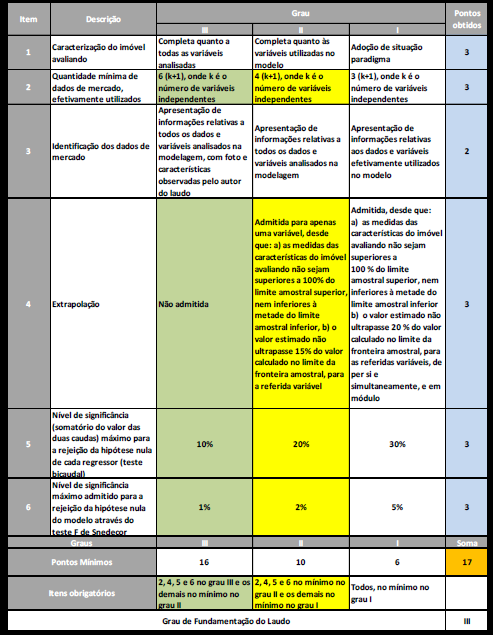
\includegraphics[width=0.947\linewidth]{figura/screenshot038}
	\label{fig:screenshot038}\\{ Fonte: Elaborado pelos Autores, pelo SISDEA}
\end{figure}
\begin{comment}
	FUNDAMENTAÇÃO\\ 
	Item Descrição		III	Grau	I	Pontos obtidos\\ 
	1	Caracterização do imóvel avaliando	Completa quanto a todas as variáveis analisadas	Completa quanto às variáveis utilizadas no modelo	Adoção de situação paradigma	3\\ 
	2	Quantidade mínima de dados de mercado, efetivamente utilizados	6 (k+1), onde k é o número de variáveis independentes	4 (k+1), onde k é o número de variáveis independentes	3 (k+1), onde k é o número de variáveis independentes	3\\ 
	Identificação dos dados de mercado	Apresentação de informações relativas a todos os dados e variáveis analisados na modelagem, com foto e características observadas pelo autor do laudo	Apresentação de informações relativas a todos os dados e variáveis analisados na modelagem	Apresentação de informações relativas aos dados e variáveis efetivamente utilizados no modelo	2\\ 
	4	Extrapolação	Não admitida	Admitida para apenas uma variável, desde que: a) as medidas das características do imóvel avaliando não sejam superiores a 100\% do limite amostral superior, nem inferiores à metade do limite amostral inferior, b) o valor estimado não ultrapasse 15\% do valor calculado no limite da fronteira amostral, para a referida variável	Admitida, desde que: a)	as medidas das características do imóvel avaliando não sejam superiores a 100 \% do limite amostral superior, nem inferiores à metade do limite amostral inferior b)	o valor estimado não ultrapasse 20 \% do valor calculado no limite da fronteira amostral, para as referidas variáveis, de per si e simultaneamente, e em módulo	3\\ 
	Nível de significância (somatório do valor das duas caudas) máximo para a rejeição da hipótese nula de cada regressor (teste bicaudal)	10\%	20\%	30\%	3\\ 
	6	Nível de significância máximo admitido para a rejeição da hipótese nula do modelo através do teste F de Snedecor	1\%	2\%	5\%	3\\ 
	Graus III				Soma\\ 
	Pontos Mínimos	16	10	6	17\\ 
	I	tens obrigatórios	2, 4, 5 e 6 no	  grau III e os demais no mínimo no grau II	2, 4, 5 e 6 no mínimo no grau II e os demais no mínimo no grau I	Todos, no mínimo no grau I	\\ 
	Grau de Fundamentação do Laudo		
\end{comment}
